\label{Sec:Rv_Analysis}
    In this section, we use the estimated parameters from the
previous section to analyze model in \Cref{model1} and the effect of the
vaccine. Some plausible scenarios are presented, depending on the effectiveness
of the vaccine, as well as the rate of vaccination.

    In the first instance, it has been shown that the interest region
of the state variables of the system is positively invariant and the proof can
be found in Appendix B.

    An important concept in the analysis of the spread of diseases is
the basic reproductive number, defined as the number of secondary
infections produced by a typical infected individual, throughout his
infectious period, when in contact with a totally susceptible population.
Following the works in \cite{Diekmann1990, Van2002}, the basic reproduction
number for system in \Cref{model1} results (see Appendix B)

\begin{equation}
    \label{Rv}
    R_{V} = R_S + R_A
\end{equation}
with
\begin{eqnarray*}
    R_S &=&
    \frac{p\beta_S\delta_E(\mu+\delta_V+(1-\epsilon)
        \lambda_V)}{(\mu+\delta_E)(\mu+\delta_V+\lambda_V)(\mu+\alpha_S)}
    \\
    R_A &=& \frac{(1-p) \beta_A \delta_E (\mu + \delta_V +
    (1-\epsilon)
        \lambda_V)}{(\mu+\delta_E)(\mu + \delta_V + \lambda_V)(\mu
        + \alpha_A )}
\end{eqnarray*}
    Note that each term of $ R_ {V} $ represents the contribution
    of the
symptomatic and asymptomatic infected, respectively, to the spread
of the
disease. Following ideas of Alexander et. al. \cite{Alexander2004},
we can
rewrite $R_V$ as
%
\begin{equation}
    \label{Rv2}
    R_{V} = R_0
        \left(
            1- \frac{\epsilon \lambda_V}{
                (\mu+\delta_V+\lambda_V)
            }
        \right)
\end{equation}
where
\begin{equation}\label{R0}
    R_0 =
        \frac{p\delta_E\beta_S}{(\mu+\delta_E)(\mu+\alpha_S)}c +
        \frac{
            (1-p) \delta_E \beta_A
        }{(\mu+\delta_E)(\mu + \alpha_A)}
¸\end{equation}
is the basic reproduction number of the system without vaccination.
Note that
$$
    \left(1- \frac{\epsilon
    \lambda_V}{(\mu+\delta_V+\lambda_V)}\right)<1.
$$
Therefore, this factor, which enclose the
parameters corresponding to the application of the vaccine,
allow us to modulate the value of $ R_0 $. In the
first instance, if $ R_0 <1 $, then $ R_V <1 $. But, if $ R_0> 1 $,
we ask if the application of the vaccine can lower $R_V$ value
below 1. In this sense, it is easy to prove that, if
\begin{equation}\label{condition1}
    \lambda_V>\frac{(R_0-1)(\mu+\delta_V)}{(\epsilon-1)R_0+1},
\end{equation}
for $\epsilon>1-(1/R_0)$, it is possible to reduce the
value of $ R_V $ below one. That is, there is a region in the
parameter space in which it is possible to reduce the value of
$ R_V $ below one, considering adequate efficacy, vaccination rate
and duration of the effect of the
vaccine. However, if the inequality in \Cref{condition1} is not
satisfied, it will not be possible to reduce the value of $ R_V $
below 1.

To illustrate the aforementioned, \Cref{R0-2D} shows the regions
where it is possible to reduce the value of $ R_V $. In this case,
we set all the system parameters as given in
\Cref{tbl:fixed_parameters} and with $ \delta_V = 1/180 $, leaving
$ \epsilon $ and $ \lambda_V $ free.
%
\begin{table}[h!]
    \begin{center}
        \begin{tabular}{rl}
            \toprule
            Parameter & Value
            \\
            \midrule
            $\beta_S$ & $0.363282$
            \\
            $\beta_A$ & $0.251521$
            \\
            $\alpha_{S}$  & $0.0925069$
            \\
            $\alpha_{A}$ & $0.167504$
            \\
            $\delta_{E}$ & $0.196078$
            \\
            $\delta_{R}$ & $0.00273973$
            \\
            $\mu$        & $0.0000391389 $
            \\
            $\theta$        & $0.11 $
            \\
            $p$        & $0.1213 $
            \\
            \bottomrule
        \end{tabular}
        \caption{Fixed parameters values of system~\eqref{model1}.
        The
        parameters corresponding to vaccination are established in
        each scenery
        studied.}
        \label{tbl:fixed_parameters}
    \end{center}
\end{table}
%
\begin{figure}[!h]
    \centering
    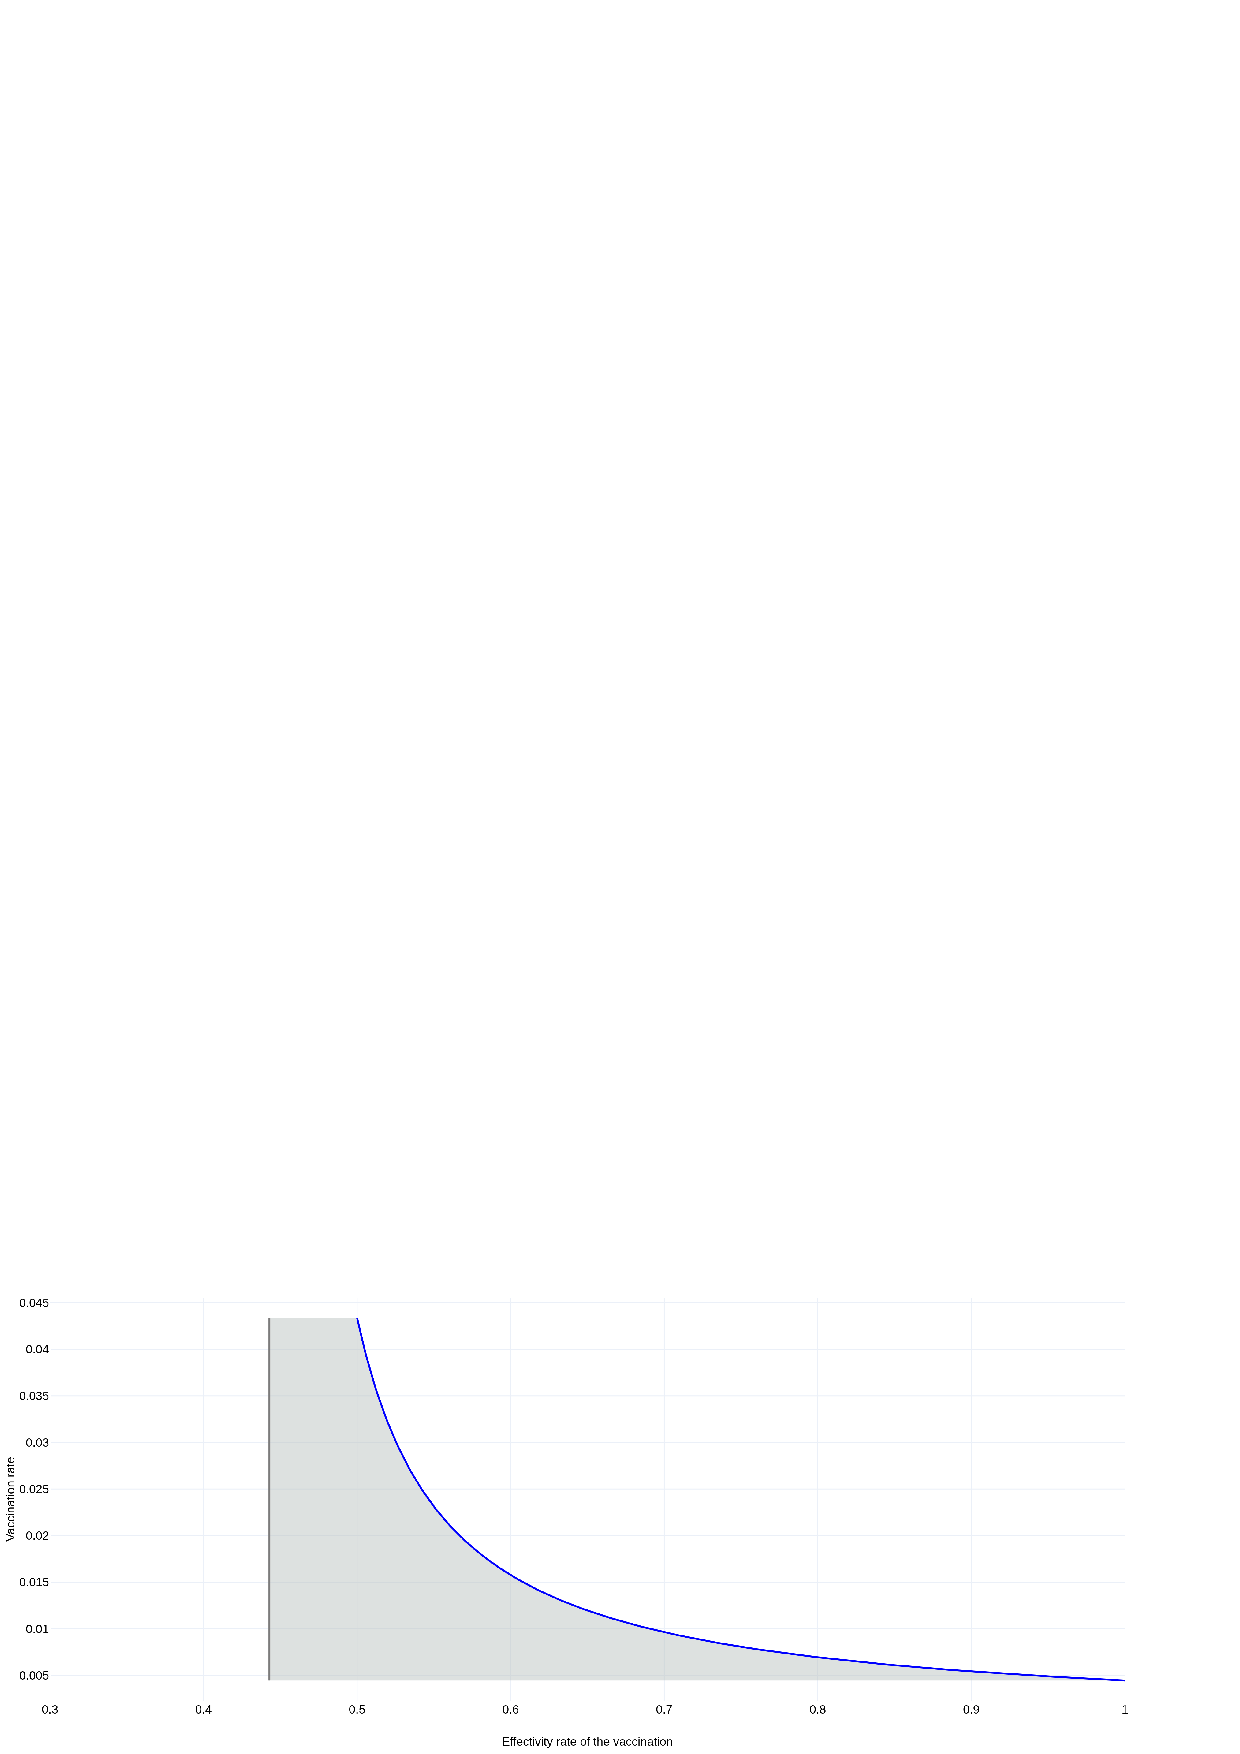
\includegraphics[width=0.7\textwidth]{R0-2D.png}
    \caption{
        In the shaded region $ R_V> 1 $ and in the white
        region $ R_V <1$. Note that, for our scenario, with a $50$
        percent vaccine effectiveness and an adequate vaccination rate,
        it is possible to reduce the $ R_V $ value below one. The orange region
        is unfeasible.
    }
    \label{R0-2D}
\end{figure}
On the other hand, vaccination policies to reach a given coverage
of a certain percentage of the population in a given period is of
great importance.
In this sense, we refer to this vaccination constant rate as the
base vaccination rate, denoted by $ \lambda_{Vbase}$.
Denote the class of total unvaccinated population at time $t$ by
$U(t)$, and assume that we remove individuals at constant rate
$\lambda_{Vbase}$ proportional to the actual population, then $U$
satisfies the initial value problem
\begin{align*}
    \dot{U} =-\lambda_{Vbase} U,
        \text{ with}
        \qquad
        U(0)=1
\end{align*}
or $U(t)=e^{-\lambda_{Vbase}t}$. Thus the number of
vaccinated individuals at time $t$ is given by
$V(t)=1-e^{-\lambda_{Vbase}t}$.
Then, to reach a coverage $x_{coverage}$ at a horizon time $T$, we
see that
$\lambda_{Vbase}$ satisfies the equation
\begin{equation}
    \label{eqn:lambda_base}
    x_{coverage} = 1 - \exp(-\lambda_{Vbase} T) \qquad\qquad
    \textrm{or}
    \qquad\qquad \lambda_{Vbase} = \frac{-\ln{(1-x_{coverage})}}{T}
\end{equation}
    Observe that in this calculation, $\lambda_{Vbase}$, it is
considered all the population to be vaccinated. Clearly,
vaccination is not applied to infective
symptomatic individuals. Therefore, \Cref{eqn:lambda_base}
represents an approximation of the vaccination scheme at constant
rate.

    On the other hand, vaccination policies to carry out the
application of the same is of utmost importance. Among other
factors, the vaccination rate at which the vaccine must be applied
in order to achieve a certain coverage of the population within a
certain horizon time must be considered. In this sense, we
will refer to this vaccination rate as the base vaccination rate
and we will denote it as $ \lambda_{Vbase}$.

    That is, $\lambda_V$ denotes the constant vaccination rate to
cover  a fraction $x_{coverage}$ in time horizon $T$. So,
\Cref{R0_contour}, shows the contour curves for $ R_0 $ considering
it as a function of the efficacy of the vaccine $ (\epsilon) $ and
of the vaccination rate $ (\delta_V) $, considering an
immunity period induced by the vaccine of half year . The blue
line, correspond to the values of $\lambda_{Vbase}$ and we can see
that with this vaccination rate, no matter how effective the
vaccine is, it is not possible to reduce the value of $R_V$ below
one. Purple lines show a scenario in which it is possible
to reduce the $R_V$ value below one, considering a vaccine efficacy
of \num{0.8} and a vaccination rate of \num{0.7}. The figure shows plausible
combinations of $\epsilon$ and $\lambda_V$ values in order to reduce the value
of $R_V$ below one.

Note that a vaccine efficacy of \SI{50}{\percent} or more is
required so that, with an adequate vaccination rate, the $R_V$
value can be reduced below one.

\begin{figure}[!h]
    \centering
    \includegraphics[scale=.50]{R0_contour.png}
    \caption{
        Contour plot  of $R_V$ like function of $ \epsilon $
        and $ \lambda_V $ and with immunity average time by
        vaccination of half year. Blue line represents the value of
        $\lambda_{Vbase} = \num{0.000611}$,
        corresponding to a coverage $x_{coverage}=0.2$ and a
        horizon time $T=365$.
        Purple lines show a scenario in which it is possible to
        reduce the $R_V$ value below one, considering a vaccine
        efficacy of \num{0.8} and a vaccination rate of \num{0.7}.
    }
    \label{R0_contour}
\end{figure}

    In the next section, the optimal control theory will be applied
to propose optimal vaccination dynamics that minimize the
number of cases of symptomatic infection and deaths due to the
disease.